\documentclass[a4paper]{article}

\usepackage[english]{babel}
\usepackage[utf8]{inputenc}
\usepackage{amsmath}
\usepackage{graphicx}
\usepackage[colorinlistoftodos]{todonotes}
\usepackage{cite}
\usepackage{float}
\usepackage{hyperref}

\title{Actividades Maestría, segundo semestre 2016}

\author{Manuel Felipe Pineda L ~ 1093223607}

\date{\today}

\begin{document}
\maketitle

\section{Estudiar las diferentes medidas de distancia entre
modelos ocultos de Markov, propuestas en la literatura.}
\label{sec:introduction}

\textbf{Notación:} Un modelo oculto de Markov será descrito como:
$\mathbf{\lambda_{i}} = \{\mathbf{u}, \mathbf{A}, \mathbf{B}\}$, donde
\textbf{u} es el vector de probabilidad del estado inicial, \textbf{A}
es la matriz de transición, y \textbf{B} es la matriz de probabilidad
de emisión. \\

Se analizaron algunas medidas de distancia basadas en diferentes criterios:

\begin{itemize}
  \item Enfoque probabilístico basado en el número (o distancia)
    de Kullback-Leibler \cite{1985} \cite{1995calculation} \cite{2005probabilistic}: $D_{KL}(\lambda_0, \lambda)$

  \item Distancia euclidiana en la probabilidad de emisión
    \cite{1995calculation} : $D_{ec}(\lambda_0, \lambda)$ y
    $D_{mec}(\lambda_0, \lambda)$

  \item Probabilidad de co-emisión para modelos ocultos de Markov
    tipo left-right  \cite{1999metrics}

  \item Probabilidad de error de Bayes \cite{2001measuring}
\end{itemize}

Los dos primeros enfoques permiten establecer medidas de distancia
entre modelos discretos para cadenas ocultas de Markov de primer
orden, a diferencia del tercer método que presenta una medida de
distancia sólo para un tipo particular de cadenas de Markov
(left-right). Sin embargo, el segundo método y su generalización
descrita en \cite{1995calculation} no tienen en cuenta los estados
ocultos de la cadena de Markov, lo cual hace posible encontrar dos
HMMs muy diferentes cuya distancia sea muy pequeña.

En el cuarto enfoque, se define la distancia entre dos modelos
basados en métodos de clasificación, estos a su vez se basan en
minimizar la probabilidad de error dado un conjunto de entrenamiento.

\subsection{Simulación Monte Carlo para evaluación de la distancia}

La distancia $D_{KL}$ está basada en encontrar la diferencia de
la probabilidad de una observación particular de emisiones, para
dos modelos diferentes, más formalmente:

$$
  \log P(\mathbf{O} \mid \lambda_1) - \log P(\mathbf{O} \mid \lambda_2)
$$

Esta probabilidad se puede encontrar para un camino de $N + 1$ estados
ocultos $S$ como:

$$
P(\mathbf{0} \mid \lambda, S) = \mathbf{u_{s_0}} \prod_{i = 1}^{N}
  \mathbf{A}_{s_{i - 1}, s_{i}} \mathbf{B}_{s_i, O_i}
$$

Usando programación dinámica, es posible encontrar la
probabilidad de las observaciones $\mathbf{O}$ para todos los posibles
caminos de $N + 1$ estados ocultos, lo cual será denotado como:

$$
\mu(\mathbf{O} \mid \lambda)
$$

Dado esto es posible evaluar $D_{KL}(\lambda_0, \lambda)$ generando
diferentes secuencias de observaciones de longitud $T$ a partir
del modelo $\lambda_0$ y finalmente evaluar la función $\mu$
para obtener la distancia:

$$
D_{KL}(\lambda_0, \lambda) =
\frac{1}{T} (\log \mu(\mathbf{O} \mid \lambda_0) -
\log \mu(\mathbf{O} \mid \lambda))
$$

\section{Implementar por lo menos dos de estas medidas en Python}
\label{sec:theory}

\begin{figure}[H]
  \centering
  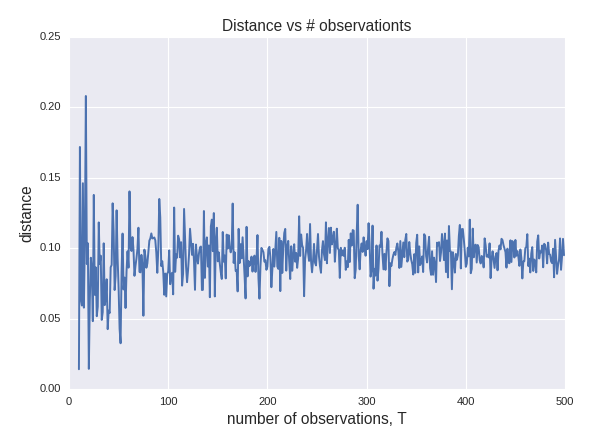
\includegraphics[width=0.9\textwidth]{./img/dist_conver3.png}
  \caption{\label{fig:conver} Distancia $D(\lambda_0, \lambda)$ vs el numero de observaciones}
\end{figure}
\subsection{Distancia $D_{KL}$}

Se implementó la distancia $D_{KL}$ y se evaluó con los modelos
provistos en \cite{1985}, en la figura \ref{fig:conver} se observa la
convergencia de la distancia en la medida que incrementa el
número de observaciones.

\begin{figure}
  \centering
  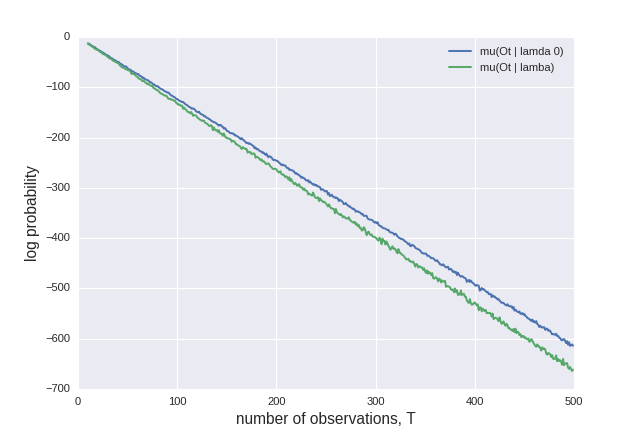
\includegraphics[width=0.9\textwidth]{./img/log_prob3.png}
  \caption{\label{fig:logprob} logaritmo de la probabilidad $\mu(O \mid \lambda_0)$ y  $\mu(O \mid \lambda)$ definido en \cite{1985}}
\end{figure}

En la figura \ref{fig:logprob} se compara el logaritmo de las
probabilidades  $\mu(O \mid \lambda_0)$ y $\mu(O \mid \lambda)$
obteniendo resultados similares a los de \cite{1985}

\subsection{Distancia euclidiana}

Se implementó también $D_{ec}$ como se define en \cite{1995calculation}

\subsection{Distancia $\widetilde{D}_{vit}$}

En \cite{1995calculation} se propone una variante para $D_{KL}$ la
cual no se enfoca en todos los posibles caminos para una observación,
sino en el camino que maximiza la probabilidad de esa observación. Este
camino es conocido como el \textit{Viterbi path}. La implementación
de esta distancia sería muy similar a $D_{KL}$ usando una simulación
por Monte Carlo y programación dinámica, debido a esto se decide
implementar la aproximación propuesta , eq. (6) de
\cite{1995calculation} denotada como $\widetilde{D}_{vit}$

\subsection{Valores obtenidos}

En esta sección se presentan los valores obtenidos en los
métodos implementados para los siguientes modelos:

$$
\mathbf{A_0} =
\begin{bmatrix}
  0.8 & 0.15 & 0.05 & 0 \\
  0.07 & 0.75 & 0.12 & 0.06 \\
  0.05 & 0.14 & 0.8 & 0.01 \\
  0.001 & 0.089 & 0.11 & 0.8
\end{bmatrix}
$$

$$
\mathbf{B_0} =
\begin{bmatrix}
  0.3 & 0.4 & 0.2 & 0.1 \\
  0.5 & 0.3 & 0.1 & 0.1 \\
  0.1 & 0.2 & 0.4 & 0.3 \\
  0.4 & 0.3 & 0.1 & 0.2
\end{bmatrix}
$$

$$
\mathbf{u_0} =
\begin{bmatrix}
  0.75 & 0.15 & 0.05 & 0.05
\end{bmatrix}
$$

y

$$
\mathbf{A_1} =
\begin{bmatrix}
  0.4 & 0.25 & 0.15 & 0.2 \\
  0.27 & 0.45 & 0.22 & 0.06 \\
  0.35 & 0.14 & 0.4 & 0.11 \\
  0.111 & 0.119 & 0.23 & 0.54
\end{bmatrix}
$$

$$
\mathbf{B_1} =
\begin{bmatrix}
  0.1 & 0.15 & 0.65 & 0.1 \\
  0.2 & 0.3 & 0.4 & 0.1 \\
  0.3 & 0.3 & 0.1 & 0.3 \\
  0.15 & 0.25 & 0.4 & 0.2
\end{bmatrix}
$$

$$
\mathbf{u_1} =
\begin{bmatrix}
  0.4 & 0.25 & 0.15 & 0.2
\end{bmatrix}
$$

\begin{table}[H]
\centering
\begin{tabular}{l|c|c}
  Método & Distancia & varianza \\\hline
  $D_{KL}$ & 0.0941689081332 & 0.000283555697027\\
  $D_{ec}$ & 0.475657439761 & \\
  $\widetilde{D}_{vit}$ & -0.694147287288 &
\end{tabular}
\caption{\label{tab:widgets}Valores obtenidos}
\end{table}

Vale la pena resaltar que $\widetilde{D}_{vit}$ presenta
problemas de estabilidad numérica ya que su evaluación requiere
calcular el logaritmo de las entradas de $\mathbf{A}$ y de
$\mathbf{B}$ las cuales podrían ser cero, como en el ejemplo usado.

\section{Implementar una medida de distancia entre modelos ocultos de Markov empleando embebimientos en Espacios de Hilbert}

\begin{verbatim}
http://www.cs.cmu.edu/~ggordon/song-boots-siddiqi-gordon-smola-hilbert-space-hmm.pdf

http://www.jmlr.org/papers/volume11/sriperumbudur10a/sriperumbudur10a.pdf

http://www.kyb.mpg.de/fileadmin/user_upload/files/publications/attachments/ALT-2007-Gretton_[0].pdf

https://www.cs.cmu.edu/~epxing/Class/10708-14/scribe_notes/scribe_note_lecture22.pdf
\end{verbatim}

\bibliography{mybib}{}
\bibliographystyle{unsrt}

\end{document}
